\apendice{Documentación de usuario}

\section{Introducción}

En esta sección se explicará todo lo necesario para que los usuarios sean capaces de instalar y usar la aplicación Android de manera correcta.

\section{Requisitos de usuarios}

Para usar la aplicación, el usuario necesita un dispositivo móvil con una versión de Android igual o superior al nivel de API 21 \ref{figVersionesAndroid}. Si se intenta instalar en una versión anterior a esta, no se garantiza el correcto funcionamiento de la aplicación.

\begin{figure}[h]
    \begin{center}%
        \begin{center}%
          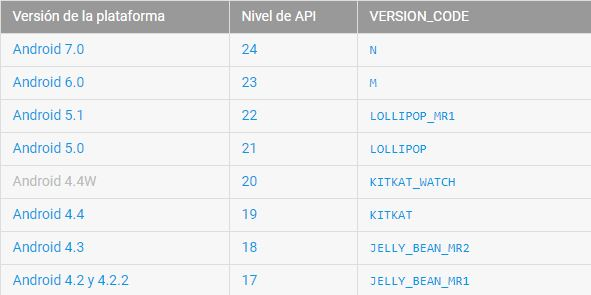
\includegraphics[width=0.8\textwidth]{imagenesAnexos/imagenesManualUsuario/VersionesAndroid}%
          \caption{Versiones de Android.}%
          \label{figVersionesAndroid}%
        \end{center}%
  	\end{center}%
\end{figure}%

\newpage
\section{Instalación}

Para instalar la aplicación solo deberemos ejecutar el fichero \textit{Ubusetas1.0.apk} que podemos encontrar en \textbackslash \textit{Binarios}\textbackslash \textit{aplicación Android}, en el dispositivo móvil.

\begin{figure}[h]
    \begin{center}%
        \begin{center}%
          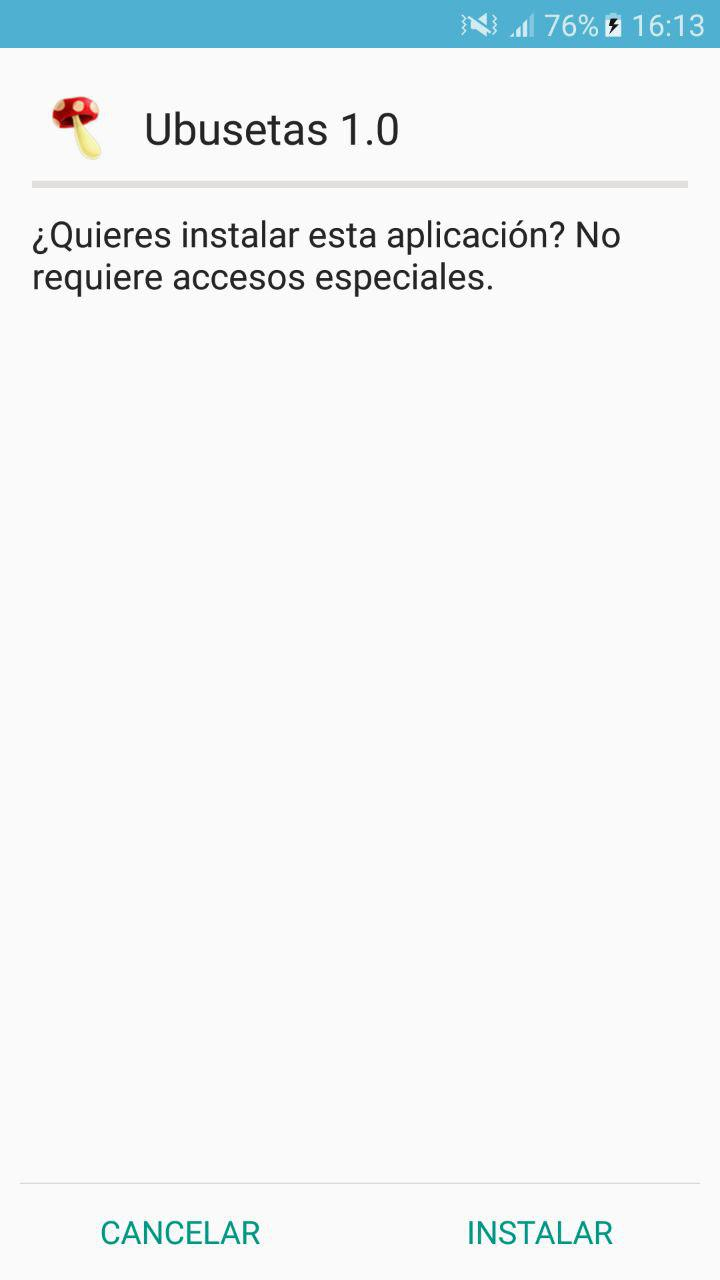
\includegraphics[width=0.4\textwidth]{imagenesAnexos/imagenesManualUsuario/InstalacionAplicacion}%
          \caption{Instalación Ubusetas1.0.}%
          \label{figInstalacionAplicacion}%
        \end{center}%
  	\end{center}%
\end{figure}%

\section{Manual del usuario}

Actualmente la aplicación cuenta con una ayuda integrada que puede ser accedida por el usuario en cualquier momento. Esta ayuda explica el funcionamiento de la actividad en la que se encuentre el usuario en ese momento.

A continuación se explicará la funcionalidad de las diferentes actividades y del menú. En el apartado \ref{disenoProcedimental} \textit{diseño procedimental} podemos encontrar los pasos necesarios para realizar las operaciones más importantes de la aplicación.

\subsection{Actividad lanzadora}

La actividad lanzadora \ref{figActividadLanzadora} es la primera página que se muestra al usuario cuando inicia la aplicación. Tiene los siguientes elementos:

\begin{itemize}
	\item Botón \textit{clasificar}: Al pulsar este botón se nos redirigirá a la actividad Recoger foto, en la cuál podremos introducir la imagen que queremos clasificar.
	\item Botón \textit{mostrar setas}: Si pulsamos este botón aparecerá un listado de las setas disponibles en la aplicación para mostrarnos información de esas especies.
	\item Botón \textit{Ir claves}: Con este botón podremos acceder al listado de claves dicotómicas disponibles.
\end{itemize}

Podemos abrir la ayuda de la actividad pulsando el botón que aparece en la parte superior derecha de la pantalla, formado por tres puntos verticales.

Para abrir el menú, podemos deslizar el dedo de izquierda a derecha de la pantalla o pulsar sobre el botón que se muestra arriba a la izquierda, formado por tres barras horizontales.

Para volver a la actividad anterior deberemos pulsar el botón de retroceso del móvil.

\begin{figure}[h]
    \begin{center}%
        \begin{center}%
          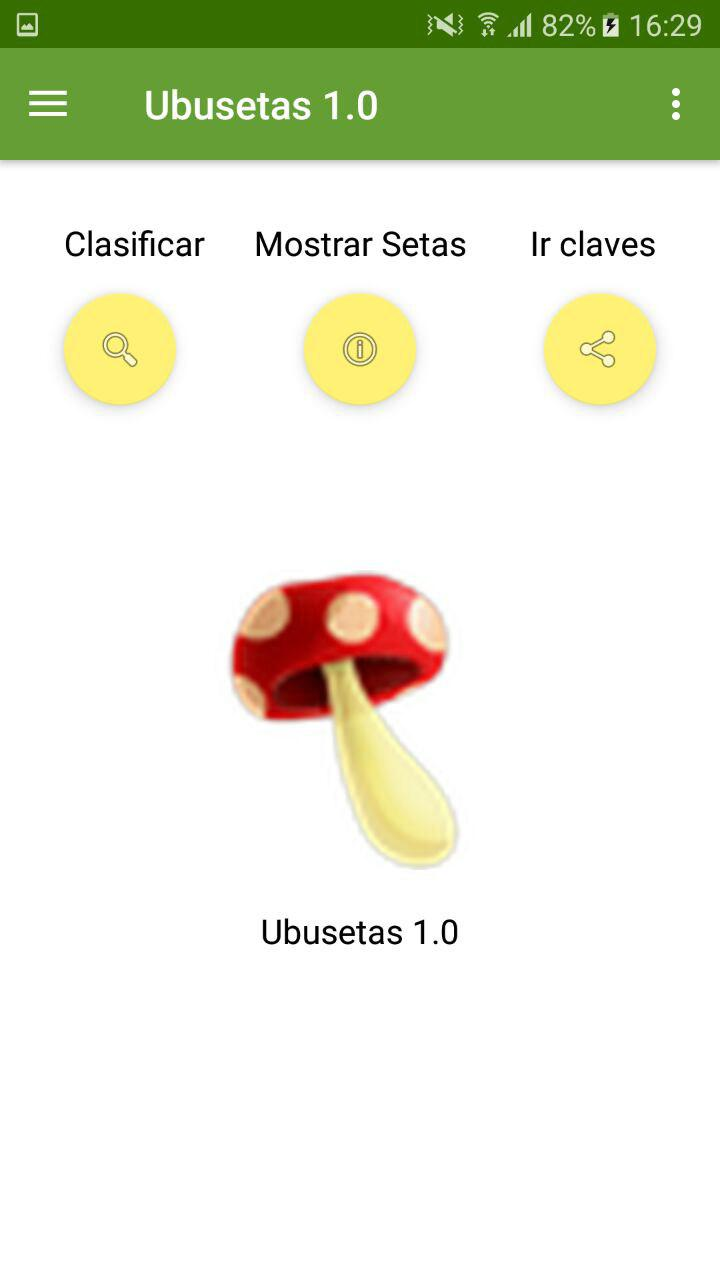
\includegraphics[width=0.5\textwidth]{imagenesAnexos/imagenesManualUsuario/ActividadLanzadora}%
          \caption{Actividad lanzadora}%
          \label{figActividadLanzadora}%
        \end{center}%
  	\end{center}%
\end{figure}%
\newpage

\subsection{Actividad recoger foto}

La actividad recoger foto \ref{figActividadRecogerFoto} nos permite introducir una imagen de una seta para ser clasificada, bien desde la galería o desde la cámara del dispositivo. Al hacer la foto desde la cámara nos aparecerá un botón por si queremos guardar la foto en la galería. Tiene los siguientes elementos:

\begin{itemize}
	\item Botón \textit{galería}: Al pulsar el icono de la galería, la aplicación nos permitirá introducir una foto desde la galería de imágenes.
	\item Botón \textit{hacer foto}: Si pulsamos el icono de la cámara de fotos podremos introducir una foto desde la cámara del móvil.
	\item Botón \textit{clasificar}: Este botón aparecerá sólo cuando hayamos introducido una foto. El icono es el de una lupa, al pulsarlo se clasificará la imagen y se nos mostrarán los resultados obtenidos.
	\item Botón \textit{guardar foto}: Este botón sólo aparece cuando introducimos una foto desde la cámara de fotos. El icono es el del disquete típico, al pulsarlo se almacenará la foto en nuestro dispositivo.
\end{itemize}

Podemos abrir la ayuda de la actividad pulsando el botón que aparece en la parte superior derecha de la pantalla, formado por tres puntos verticales.

Para abrir el menú, podemos deslizar el dedo de izquierda a derecha de la pantalla o pulsar sobre el botón que se muestra arriba a la izquierda, formado por tres barras horizontales.

Para volver a la actividad anterior deberemos pulsar el botón de retroceso del móvil.

\begin{figure}[h]
    \begin{center}%
        \begin{center}%
          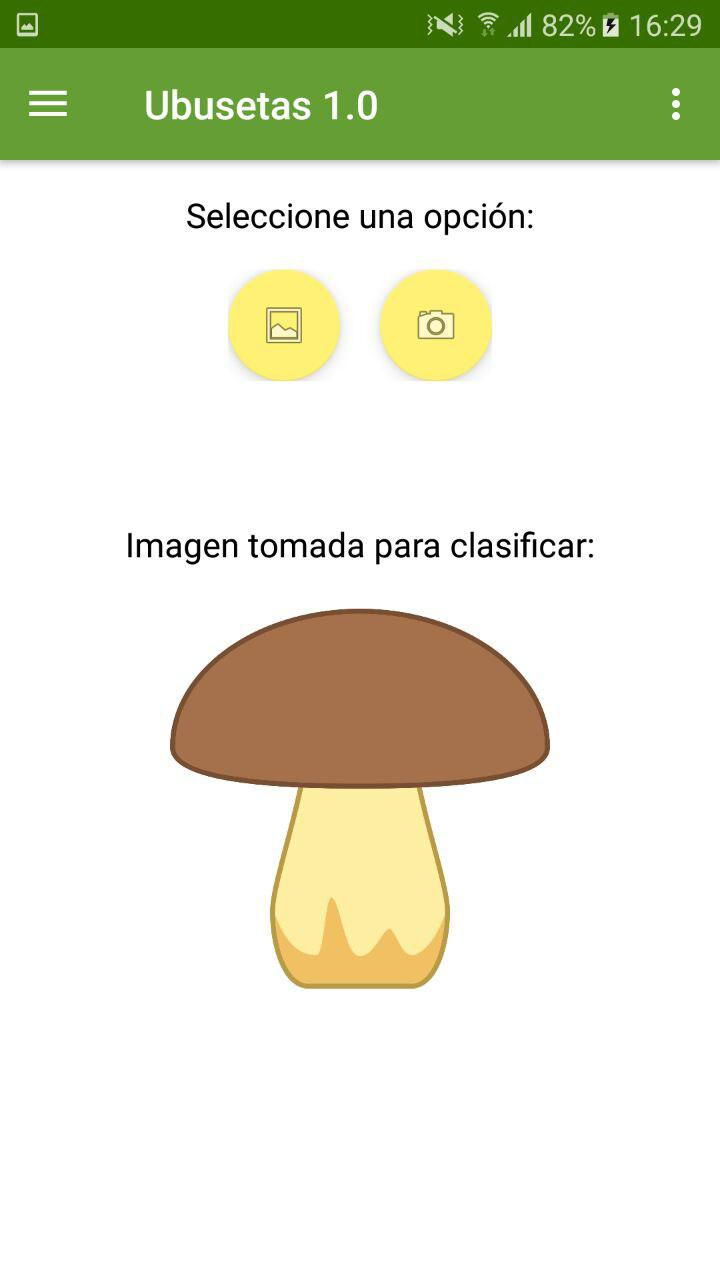
\includegraphics[width=0.5\textwidth]{imagenesAnexos/imagenesManualUsuario/ActividadRecogerFoto}%
          \caption{Actividad recoger foto}%
          \label{figActividadRecogerFoto}%
        \end{center}%
  	\end{center}%
\end{figure}%
\newpage

\subsection{Actividad mostrar resultados}

La actividad mostrar resultados \ref{figActividadMostrarResultados} aparecerá cuando hayamos clasificado una imagen. En ella se nos mostrarán los resultados de especies mas probables devueltos por el clasificador. Tiene los siguientes elementos:

\begin{itemize}
	\item Botón \textit{refrescar}: Al pulsar el icono de refrescar, se cambiará la imagen de la seta asociada a cada especie de los resultados.
	\item Botón \textit{clave dicotómica}: Si pulsamos el icono de la clave dicotómica, representado igual que el icono de compartir, se nos preguntará sobre que especies de las clasificadas queremos aplicar la clave dicotómica.
\end{itemize}

Si pulsamos un resultado, podremos comparar nuestra foto con la de la especie seleccionada.

Si mantenemos pulsado un resultado, nos aparecerá información de la especie pulsada.

Podemos abrir la ayuda de la actividad pulsando el botón que aparece en la parte superior derecha de la pantalla, formado por tres puntos verticales.

Para abrir el menú, podemos deslizar el dedo de izquierda a derecha de la pantalla o pulsar sobre el botón que se muestra arriba a la izquierda, formado por tres barras horizontales.

Para volver a la actividad anterior deberemos pulsar el botón de retroceso del móvil.

\begin{figure}[h]
    \begin{center}%
        \begin{center}%
          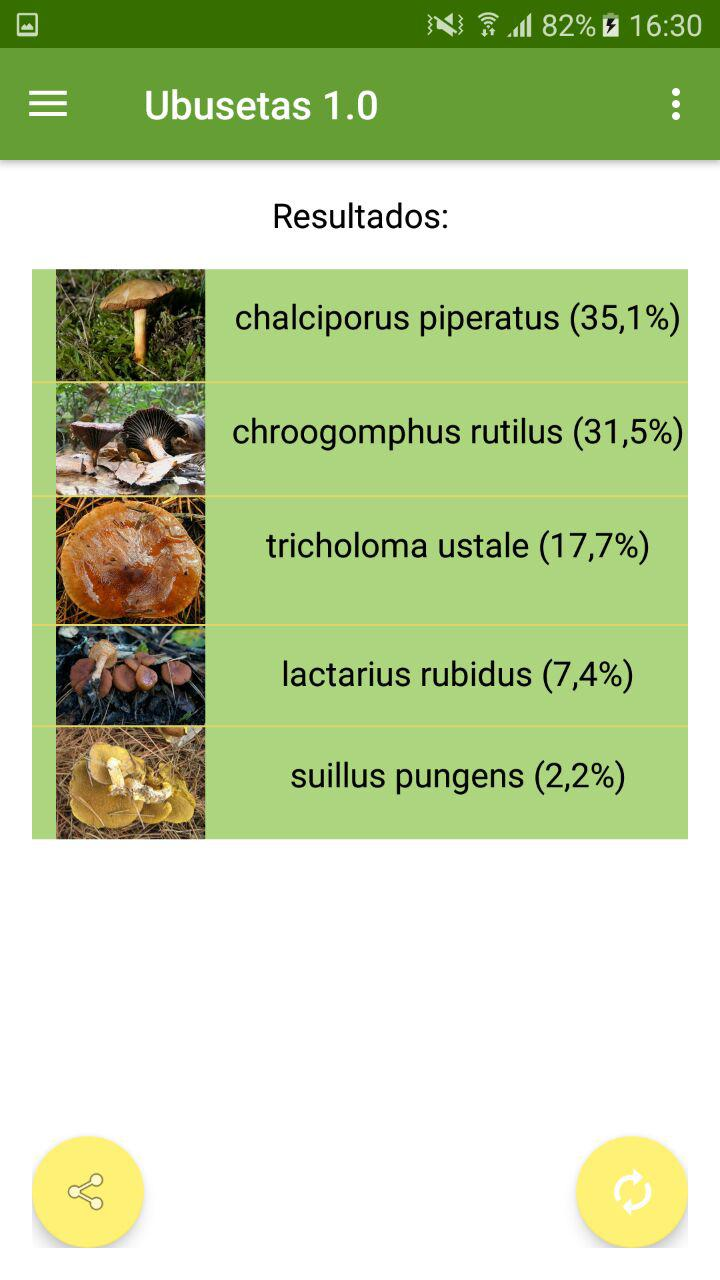
\includegraphics[width=0.5\textwidth]{imagenesAnexos/imagenesManualUsuario/ActividadMostrarResultados}%
          \caption{Actividad mostrar resultados}%
          \label{figActividadMostrarResultados}%
        \end{center}%
  	\end{center}%
\end{figure}%
\newpage

\subsection{Actividad mostrar comparativa}

La actividad mostrar comparativa \ref{figActividadMostrarComparativa} aparecerá cuando hayamos pulsado uno de los resultados de la actividad mostrar resultados. En ella se nos mostrará una imagen de la especie pulsada y nuestra imagen, podremos ampliar ambas para comparar diferencias entre ellas.

Podemos abrir la ayuda de la actividad pulsando el botón que aparece en la parte superior derecha de la pantalla, formado por tres puntos verticales.

Para abrir el menú, podemos deslizar el dedo de izquierda a derecha de la pantalla o pulsar sobre el botón que se muestra arriba a la izquierda, formado por tres barras horizontales.

Para volver a la actividad anterior deberemos pulsar el botón de retroceso del móvil.

\begin{figure}[h]
    \begin{center}%
        \begin{center}%
          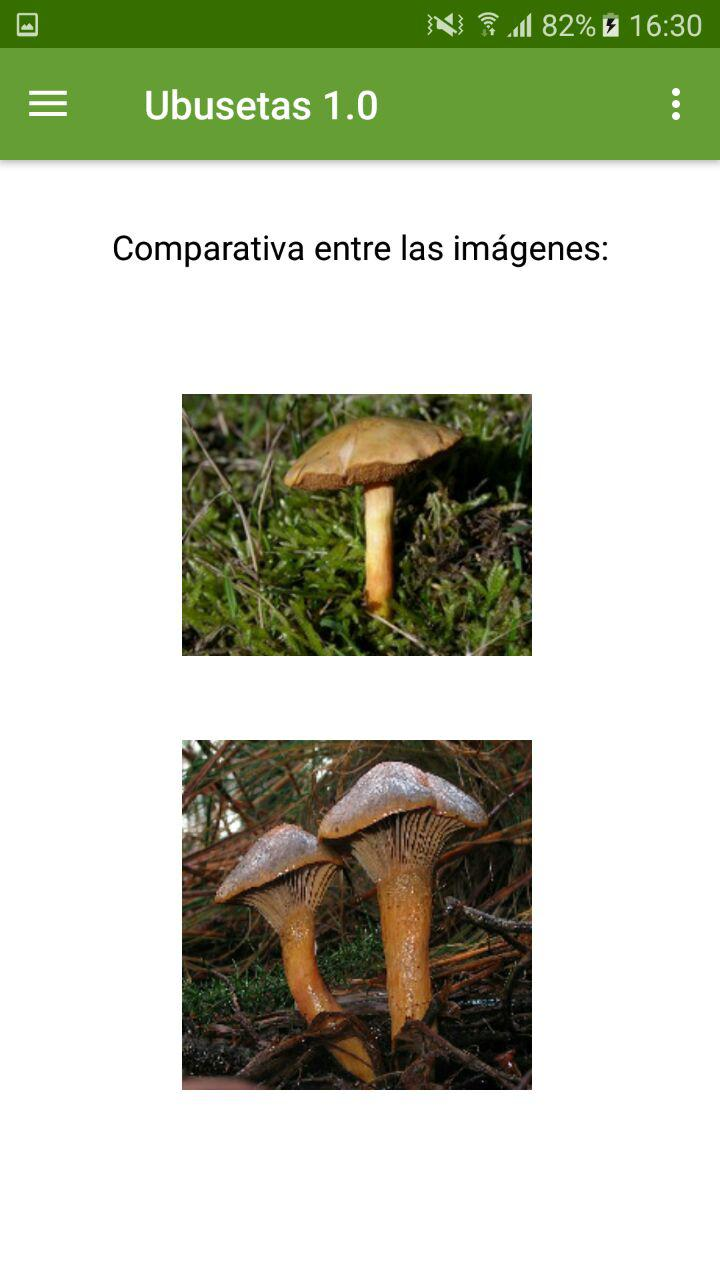
\includegraphics[width=0.5\textwidth]{imagenesAnexos/imagenesManualUsuario/ActividadMostrarComparativa}%
          \caption{Actividad mostrar comparativa}%
          \label{figActividadMostrarComparativa}%
        \end{center}%
  	\end{center}%
\end{figure}%
\newpage

\subsection{Actividad elegir claves}

La actividad elegir claves \ref{figActividadElegirClaves} nos permite elegir sobre que especies queremos que se filtre la clave dicotómica para acotar las preguntas sobre estas especies. Esto no quiere decir que la clave no pueda clasificar una especie que se encuentre entre las elegidas, sino que se acota la búsqueda teniendo en cuenta las especies seleccionadas. Para seleccionar las especies deberemos pulsar sobre ellas y después pulsar sobre el botón de seleccionar. Tiene los siguientes elementos:

\begin{itemize}
	\item Botón \textit{seleccionar}: Al pulsar sobre este botón fijaremos las especies.
	\item Botón \textit{ir clave dicotómica}: Al pulsar este botón accedemos a la clave dicotómica, deberemos haber seleccionado al menos dos especies de las disponibles. Si no queremos filtrar, deberemos elegir todas las especies.
\end{itemize}

Podemos abrir la ayuda de la actividad pulsando el botón que aparece en la parte superior derecha de la pantalla, formado por tres puntos verticales.

Para abrir el menú, podemos deslizar el dedo de izquierda a derecha de la pantalla o pulsar sobre el botón que se muestra arriba a la izquierda, formado por tres barras horizontales.

Para volver a la actividad anterior deberemos pulsar el botón de retroceso del móvil.

\begin{figure}[h]
    \begin{center}%
        \begin{center}%
          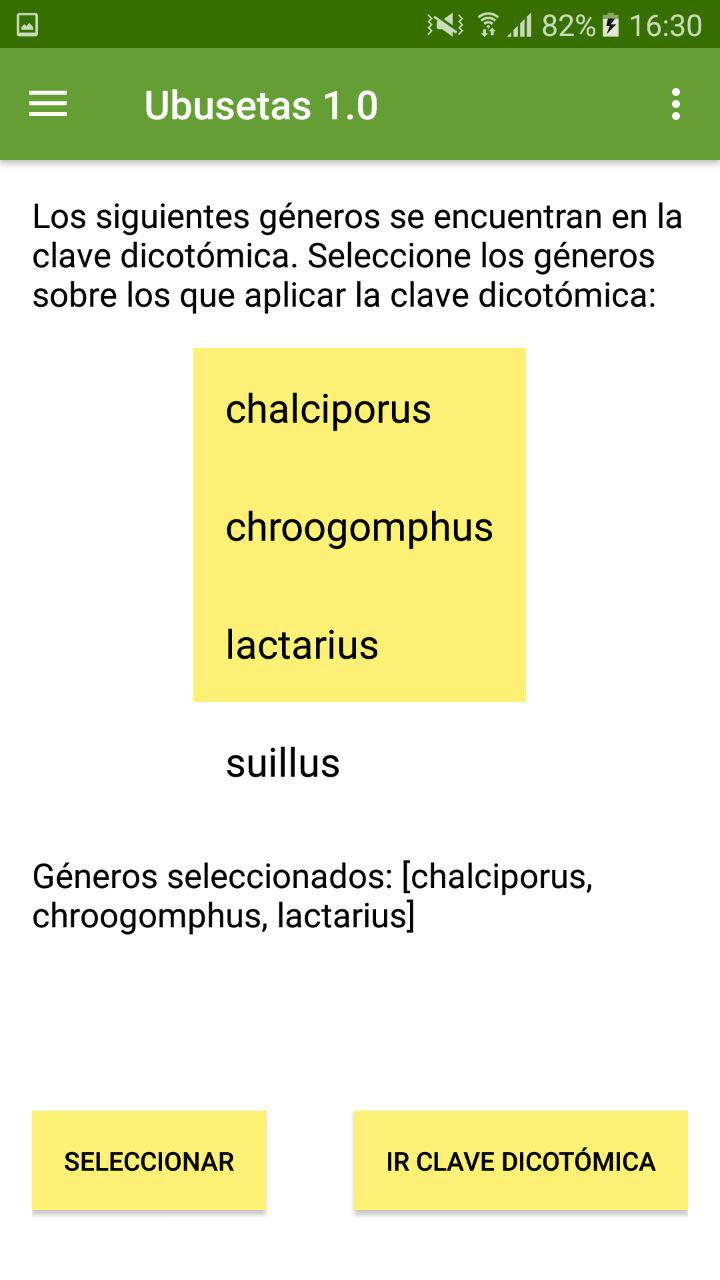
\includegraphics[width=0.5\textwidth]{imagenesAnexos/imagenesManualUsuario/ActividadElegirClaves}%
          \caption{Actividad elegir claves}%
          \label{figActividadElegirClaves}%
        \end{center}%
  	\end{center}%
\end{figure}%
\newpage

\subsection{Actividad clave dicotómica}

La actividad clave dicotómica \ref{figActividadClaveDicotomica} podrá ser accedida después de haber clasificado una imagen o después de haber seleccionado una clave de las disponibles en la actividad mostrar claves.
En esta actividad se nos irán proponiendo sentencias y deberemos elegir la que más se adecua a las características de la seta que queremos clasificar. Tiene los siguientes elementos:

\begin{itemize}
	\item Botón \textit{volver}: Nos devuelve a la pregunta anterior de la clave.
\end{itemize}

Podemos abrir la ayuda de la actividad pulsando el botón que aparece en la parte superior derecha de la pantalla, formado por tres puntos verticales.

Para abrir el menú, podemos deslizar el dedo de izquierda a derecha de la pantalla o pulsar sobre el botón que se muestra arriba a la izquierda, formado por tres barras horizontales.

Para volver a la actividad anterior deberemos pulsar el botón de retroceso del móvil.

\begin{figure}[h]
    \begin{center}%
        \begin{center}%
          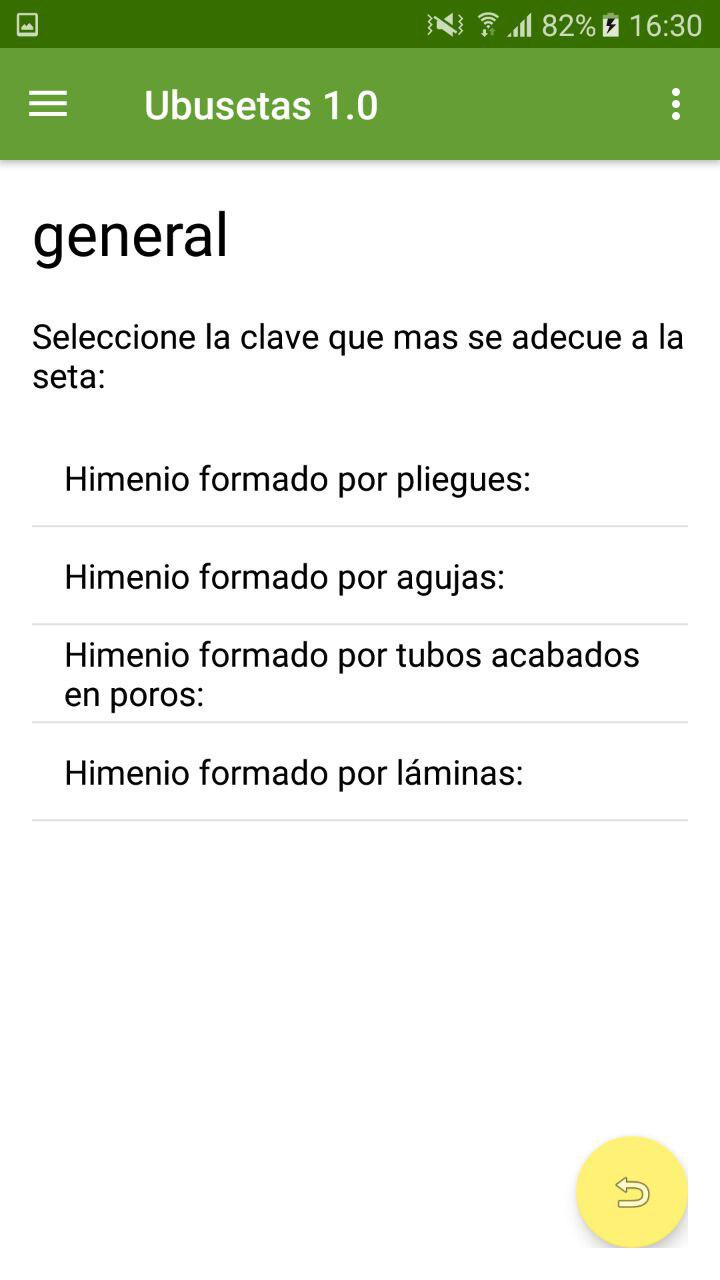
\includegraphics[width=0.5\textwidth]{imagenesAnexos/imagenesManualUsuario/ActividadClaveDicotomica}%
          \caption{Actividad clave dicotómica}%
          \label{figActividadClaveDicotomica}%
        \end{center}%
  	\end{center}%
\end{figure}%
\newpage

\subsection{Actividad mostrar claves}

La actividad mostrar claves \ref{figActividadMostrarClaves} nos mostrará un listado de las claves dicotómicas disponibles. Al pulsar una clave, se nos redirigirá a las preguntas asociadas a esa clave.

Podemos abrir la ayuda de la actividad pulsando el botón que aparece en la parte superior derecha de la pantalla, formado por tres puntos verticales.

Para abrir el menú, podemos deslizar el dedo de izquierda a derecha de la pantalla o pulsar sobre el botón que se muestra arriba a la izquierda, formado por tres barras horizontales.

\begin{figure}[h]
    \begin{center}%
        \begin{center}%
          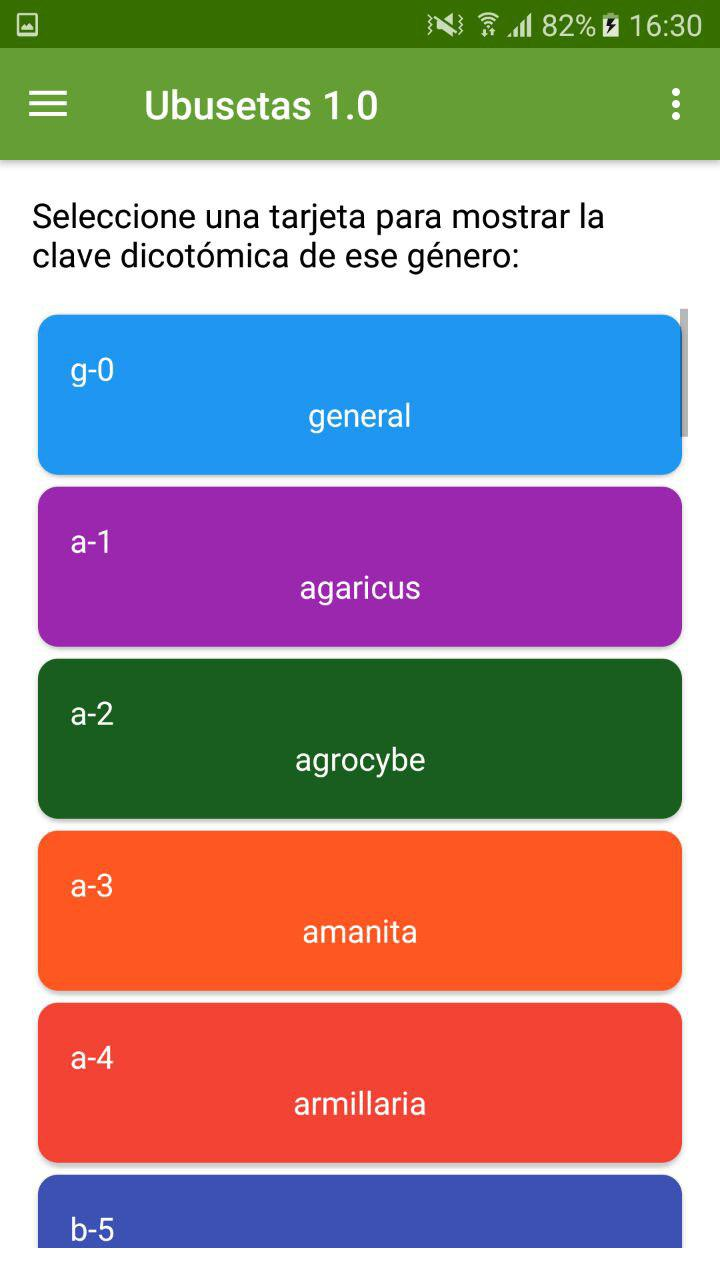
\includegraphics[width=0.5\textwidth]{imagenesAnexos/imagenesManualUsuario/ActividadMostrarClaves}%
          \caption{Actividad mostrar claves}%
          \label{figActividadMostrarClaves}%
        \end{center}%
  	\end{center}%
\end{figure}%
\newpage

\subsection{Actividad mostrar setas}

La actividad mostrar setas \ref{figActividadMostrarSetas} nos mostrará un listado de las setas disponibles. Al pulsar una especie, se nos mostrará información de esta.

Podemos abrir la ayuda de la actividad pulsando el botón que aparece en la parte superior derecha de la pantalla, formado por tres puntos verticales.

Para abrir el menú, podemos deslizar el dedo de izquierda a derecha de la pantalla o pulsar sobre el botón que se muestra arriba a la izquierda, formado por tres barras horizontales.

Para volver a la actividad anterior deberemos pulsar el botón de retroceso del móvil.

\begin{figure}[h]
    \begin{center}%
        \begin{center}%
          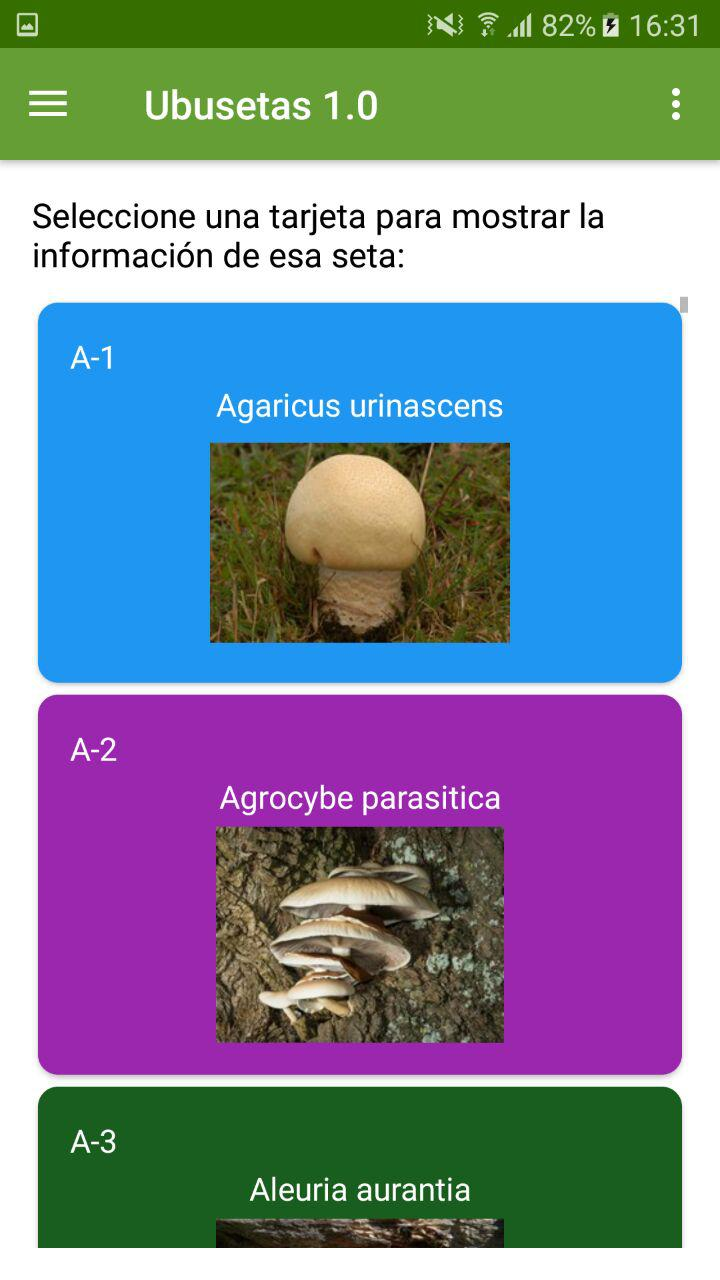
\includegraphics[width=0.5\textwidth]{imagenesAnexos/imagenesManualUsuario/ActividadMostrarSetas}%
          \caption{Actividad mostrar setas}%
          \label{figActividadMostrarSetas}%
        \end{center}%
  	\end{center}%
\end{figure}%
\newpage

\subsection{Actividad mostrar información}

La actividad mostrar información \ref{figActividadMostrarInformacion} nos proporcionará una descripción de la especie, su comestibilidad, el género al que pertenece y un link a la \textit{Wikipedia} para ampliar la información presentada.

Podemos abrir la ayuda de la actividad pulsando el botón que aparece en la parte superior derecha de la pantalla, formado por tres puntos verticales.

Para abrir el menú, podemos deslizar el dedo de izquierda a derecha de la pantalla o pulsar sobre el botón que se muestra arriba a la izquierda, formado por tres barras horizontales.

Para volver a la actividad anterior deberemos pulsar el botón de retroceso del móvil.

\begin{figure}[h]
    \begin{center}%
        \begin{center}%
          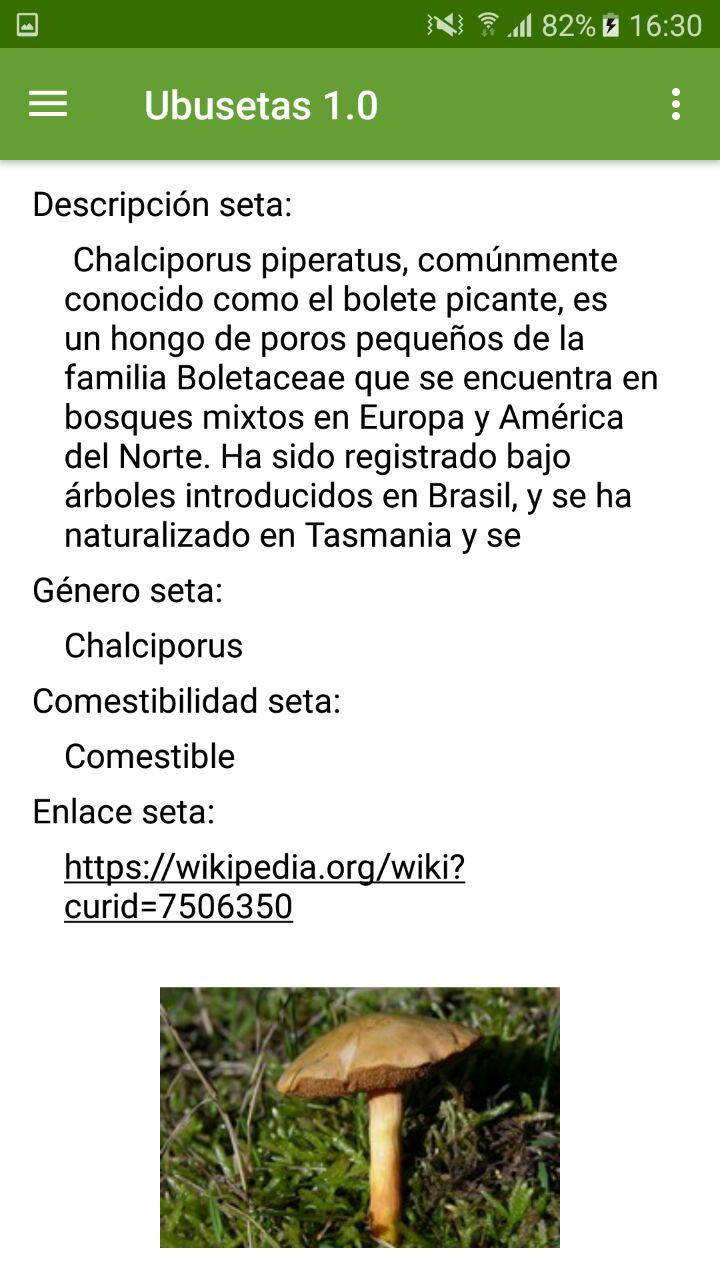
\includegraphics[width=0.5\textwidth]{imagenesAnexos/imagenesManualUsuario/ActividadMostrarInformacion}%
          \caption{Actividad mostrar información}%
          \label{figActividadMostrarInformacion}%
        \end{center}%
  	\end{center}%
\end{figure}%
\newpage

\subsection{Menú de la aplicación}

El menú \ref{figMenu} de la aplicación es accesible en cualquier pantalla de esta. Para abrir el menú, podemos deslizar el dedo de izquierda a derecha de la pantalla o pulsar sobre el botón que se muestra arriba a la izquierda, formado por tres barras horizontales. Tiene los siguientes elementos:

\begin{itemize}
	\item Botón \textit{home}: Nos lleva a la actividad principal de la aplicación.
	\item Botón \textit{clasificar}: Nos lleva a la actividad \textit{recoger foto}, que nos permite introducir la imagen para clasificar.
	\item Botón \textit{ir claves dicotómicas}: Este botón nos lleva al listado de claves dicotómicas de la aplicación.
	\item Botón \textit{información setas}: Este botón nos lleva al listado de especies de setas de la aplicación.
	\item Botón \textit{cambiar idioma}: Alterna el idioma de la aplicación entre Español e Inglés.
	\item Botón \textit{ayuda}: Despliega la ayuda del menú.
\end{itemize}

Para salir del menú podemos deslizar el dedo de derecha a izquierda por la pantalla o pulsar el botón de retroceso del móvil.

\begin{figure}[h]
    \begin{center}%
        \begin{center}%
          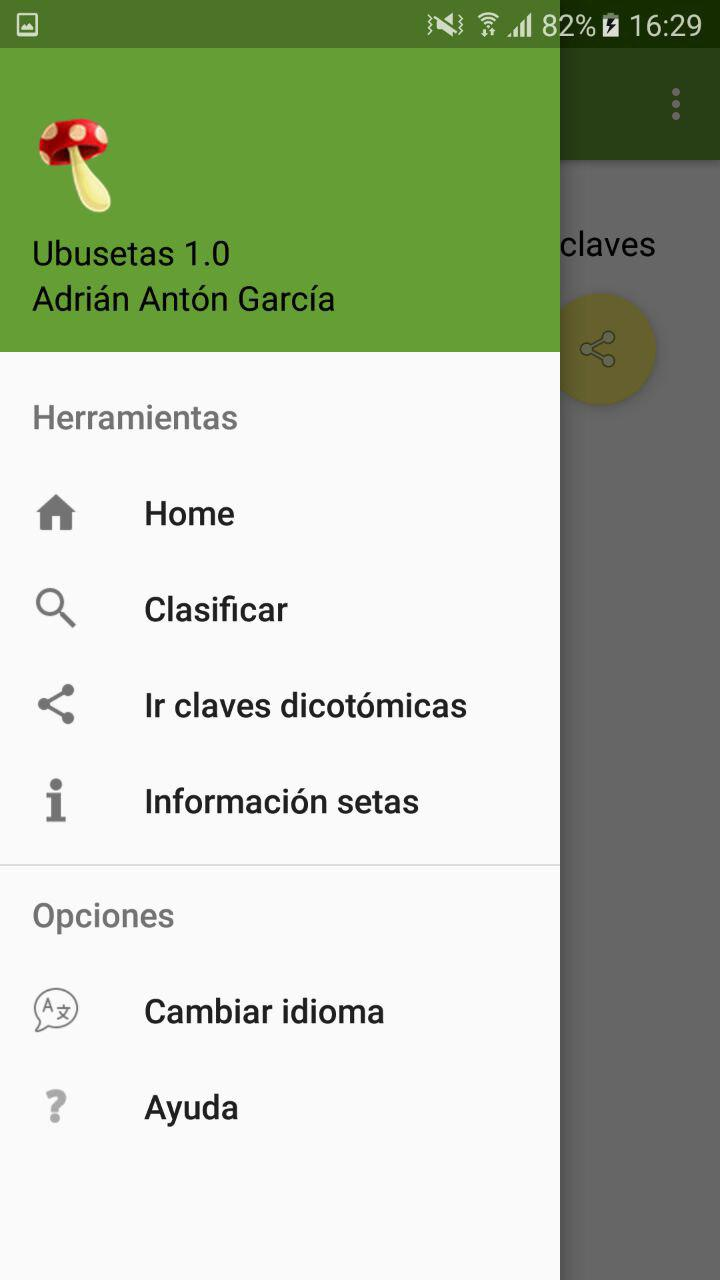
\includegraphics[width=0.5\textwidth]{imagenesAnexos/imagenesManualUsuario/Menu}%
          \caption{Menú de la aplicación}%
          \label{figMenu}%
        \end{center}%
  	\end{center}%
\end{figure}%
\newpage


